% Intrinsic-alignment scale cuts for Roman cosmic shear: NLA and TATT
% against the FLAMINGO alignment spectra. The presentable summary of the
% scale-cut work of 1 to 11 November 2026, rebuilt from the work logs in
% analysis/roman_dchi2/report/ (summary.pdf, strategies.pdf, hmc_review.pdf).
% Build with the summary-notes skill: assets/build_note.sh notes/scale_cuts_summary
\documentclass[11pt]{article}

\usepackage[margin=1in]{geometry}
\usepackage{amsmath}
\usepackage{amssymb}
\usepackage{graphicx}
\usepackage{booktabs}
\usepackage{xcolor}
\usepackage[font=small,labelfont=bf,labelsep=period]{caption}
\usepackage[hidelinks]{hyperref}

% Let figures share pages with text instead of leaving float-only pages.
\renewcommand{\topfraction}{0.85}
\renewcommand{\bottomfraction}{0.7}
\renewcommand{\textfraction}{0.12}
\renewcommand{\floatpagefraction}{0.8}

% Symbols, one macro per object.
\newcommand{\hMpc}{\,h\,{\rm Mpc}^{-1}}
\newcommand{\kmax}{k_{\rm max}}
\newcommand{\kuv}{k_{\rm UV}}
\newcommand{\dchi}{\Delta\chi^2}
\newcommand{\FoB}{{\rm FoB}}
\newcommand{\PNL}{P_{\rm NL}}
\newcommand{\PdE}{P_{\delta E}}
\newcommand{\T}{^{\mathsf{T}}}
% The clause of every caption with a K_0 axis.
\newcommand{\kuvclause}{Masks: IR/UV with $\alpha = 0.05$; $K_0$ in
  $h\,{\rm Mpc}^{-1}$.}

% =====================================================================
% Numbers
% =====================================================================
% Every number the text quotes is defined here. Part 1 holds results:
% they move when the analysis is rerun, and print in red when
% \numbersfinalfalse is set. Part 2 holds inputs (survey, simulation,
% thresholds), which a rerun does not change. Paths are relative to
% analysis/roman_dchi2/ of this repository; "strategies" is
% report/strategies.tex (10 November 2026), "hmc review" is
% report/hmc_review.tex (11 November 2026).
%
% Statements of the text that rest on Part 1; re-check each after a
% refresh:
%   - with the white term in the truth and no nuisance, NLA and TATT
%     need nearly the same cut (Summary; "The cut with the production
%     covariance");
%   - with one white-II nuisance, NLA is limited to a smaller K_0 than
%     TATT (Summary; same section);
%   - the absolute S_8 shift is nearly independent of the mask
%     ("Why cutting does not remove the bias");
%   - HMc stays below 0.3 to K_0 = 0.5 in case B on both families
%     ("A halo model with central alignment").
\newif\ifnumbersfinal
\numbersfinaltrue
\newcommand{\refresh}[1]{\ifnumbersfinal#1\else\textcolor{red}{#1}\fi}
% ---------------------------------------------------------------------
% Part 1: results.
%
% Simulation cuts (v3/cuts.csv, core snapshots): GoF k_max ranges [h/Mpc]
\newcommand{\SimNLAlo}{\refresh{0.09}}
\newcommand{\SimNLAhi}{\refresh{0.12}}
\newcommand{\SimTATTlo}{\refresh{0.22}}
\newcommand{\SimTATThi}{\refresh{0.39}}
% the same GoF rule at Roman's sensitivity, f = 0.02 to 0.04
% (v4/derived.json, volume.<model>.comb_lambda)
\newcommand{\VolNLAlo}{\refresh{0.22}}
\newcommand{\VolNLAhi}{\refresh{0.29}}
\newcommand{\VolTATTlo}{\refresh{0.39}}
\newcommand{\VolTATThi}{\refresh{0.52}}
% false-cut rate of the GoF rule per snapshot on a model truth
% (strategies, Table "calib"; v4/sim_strategies.json)
\newcommand{\FalseNLA}{\refresh{9.8}}
\newcommand{\FalseTATT}{\refresh{10.8}}
% white II excess over the core snapshots, in units of N_s (report/summary.tex,
% Table "snaps", column X/N_s)
\newcommand{\WhiteLo}{\refresh{1.5}}
\newcommand{\WhiteHi}{\refresh{3}}
% The required accuracy on the K_0 = 0.3 mask, Gaussian covariance
% (v4/roman_strategies.json, tolerance["n1:0.3"], eps_dchi1), percent
\newcommand{\ReqGIa}{\refresh{7}}
\newcommand{\ReqGIb}{\refresh{17}}
\newcommand{\ReqGIc}{\refresh{38}}
\newcommand{\ReqIIa}{\refresh{14}}
\newcommand{\ReqIIb}{\refresh{22}}
\newcommand{\ReqIIc}{\refresh{48}}
% The bias floor, Gaussian covariance (v4/derived.json, tradeoff):
% |delta S_8| range and the sigma(S_8) range of the masks
\newcommand{\FloorLo}{\refresh{1.1}}
\newcommand{\FloorHi}{\refresh{2.6}}
\newcommand{\SigmaRange}{\refresh{6.6}}
% Gaussian covariance: the K_0 of FoB = 0.3, both models (v3/mask_scan.json)
\newcommand{\GaussKzero}{\refresh{0.3}}
% Undetectability at K_0 = 0.3 (strategies, section "B3"): best-fit chi2
% and the chi2 scatter sqrt(2N) for N = 281
\newcommand{\DetectChi}{\refresh{1}}
\newcommand{\DetectScatter}{\refresh{24}}
% Production covariance (v3/mask_scan_ex1_{D1,flat}.json, case A; case B
% in brackets in the table; sigma(S_8) from report/tab_ex1.tex and the
% strategies Table "rec")
\newcommand{\ExNLAwFoB}{\refresh{0.22}}   % NLA + white, K_0 = 0.35, 1/D
\newcommand{\ExNLAwPts}{\refresh{317}}
\newcommand{\ExNLAwSig}{\refresh{0.0066}}
\newcommand{\ExTATTwFoB}{\refresh{0.24}}  % TATT + white, K_0 = 0.5, 1/D
\newcommand{\ExTATTwPts}{\refresh{385}}
\newcommand{\ExTATTwSig}{\refresh{0.0055}}
\newcommand{\ExGainSig}{\refresh{17}}     % percent smaller sigma(S_8)
\newcommand{\ExGainPts}{\refresh{21}}     % percent more points
\newcommand{\ExNLAthreeFoB}{\refresh{0.24}}  % no white, K_0 = 0.3
\newcommand{\ExTATTthreeFoB}{\refresh{0.28}}
\newcommand{\ExNLAfiveFoB}{\refresh{0.32}}   % no white, K_0 = 0.35
\newcommand{\ExTATTfiveFoB}{\refresh{0.29}}
\newcommand{\ExNLAwFour}{\refresh{0.46}}  % NLA + white, K_0 = 0.4
% Halo model (hmc review; v6/hmc_scan_ex1_*.json): FLAMINGO chi2/nu summed
% over z = 0.2 to 2 at k_max = 0.52 with the white term, HMc and TATT;
% Roman case B largest FoB of HMc to K_0 = 0.5; the TATT crossings
\newcommand{\HMcChi}{\refresh{1.04}}
\newcommand{\HMcTATTChi}{\refresh{5.73}}
\newcommand{\HMcCutLo}{\refresh{0.52}}
\newcommand{\HMcCutHi}{\refresh{0.70}}
\newcommand{\HMcMaxFoB}{\refresh{0.29}}
\newcommand{\HMcTATTcrossD}{\refresh{0.325}}
\newcommand{\HMcTATTcrossC}{\refresh{0.45}}
% MCMC projection shift of the matched TATT control at K_0 = 0.3
% (v3/mcmc_TATT_TATT.json), in sigma
\newcommand{\Projection}{\refresh{0.24}}
% ---------------------------------------------------------------------
% Part 2: inputs.
\newcommand{\Npts}{1080}
\newcommand{\Alpha}{0.05}
\newcommand{\Threshold}{0.3}

\begin{document}

\begin{center}
  {\LARGE Intrinsic-alignment scale cuts for Roman\par}
  \vspace{0.6em}
  {\large NLA and TATT against the FLAMINGO alignment spectra\par}
  \vspace{0.6em}
  {\large November 2026\par}
  \ifnumbersfinal\else
    \vspace{0.6em}
    {\color{red}Numbers in red are being refreshed.\par}
  \fi
\end{center}
\vspace{1em}

\section{Summary}
\label{sec:summary}

\paragraph{The question.}
Which scales of Roman cosmic shear can be analyzed with the NLA and
the TATT intrinsic-alignment (IA) models without biasing $(\Omega_m,
S_8)$, when the true alignments are those measured in the FLAMINGO
simulation?

\paragraph{The answer.}
The cut is defined in Roman, not in the simulation: it is the largest
mask on which the best-fit shift of $(\Omega_m, S_8)$, with every
parameter free, stays below $\Threshold\,\sigma$ in the two-dimensional
figure of bias (Section~\ref{sec:setup}). With the production
covariance and the production mask family $\kuv(z) = K_0/D(z)$, and
with one free amplitude for a white intrinsic-intrinsic (II) term that
FLAMINGO contains and neither model has, NLA is limited to $K_0 =
0.35\hMpc$ (figure of bias \ExNLAwFoB, \ExNLAwPts{} of \Npts{} points,
$\sigma(S_8) = \ExNLAwSig$) while TATT remains unbiased to $K_0 =
0.5\hMpc$ (\ExTATTwFoB, \ExTATTwPts{} points, $\sigma(S_8) =
\ExTATTwSig$, \ExGainSig\% smaller). Without the white-II amplitude
the two models need the same cut: $K_0 = 0.3$ passes for both, and
$K_0 = 0.35$ is marginal.

\paragraph{Why the simulation alone does not set the cut.}
Fitted directly to the FLAMINGO spectra, NLA fails at $\kmax \simeq
\SimNLAlo$ to $\SimNLAhi\hMpc$ and TATT at \SimTATTlo{} to
\SimTATThi$\hMpc$, nearly independently of redshift. These cuts measure
whether a residual is detectable with FLAMINGO's error bars, so they
move with the size of the simulation box. At the sensitivity Roman has
to the same residuals they become \VolNLAlo{} to \VolNLAhi{} (NLA) and
\VolTATTlo{} to \VolTATThi{} (TATT), the range of the Roman-defined
cut (Section~\ref{sec:sim}).

\paragraph{Why cutting does not remove the bias.}
FLAMINGO's II spectrum contains a white (one-halo-like) term, flat in
$k$, of \WhiteLo{} to \WhiteHi{} times the shape-noise level. A white
spectrum is a constant angular power spectrum, which puts a
$\theta^{-2}$ tail into $\xi_-$ at every angle; no cut in $k$ removes
it (Section~\ref{sec:white}). The absolute $S_8$ shift is therefore
about $2\times10^{-3}$ for every mask, and the figure of bias rises
with $K_0$ only because the error bar shrinks
(Section~\ref{sec:floor}). The shift is also invisible in the data: at
$K_0 = 0.3$ it adds $\dchi \simeq \DetectChi$ to a $\chi^2$ whose
scatter is \DetectScatter, so the cut has to be fixed from simulations
before unblinding.

\paragraph{A better model.}
A halo model in which centrals are aligned with their own triaxial
host (HMc) fits FLAMINGO to $\kmax = \HMcCutLo$ to $\HMcCutHi\hMpc$
and keeps the Roman figure of bias at or below \HMcMaxFoB{} to $K_0 =
0.5$ in both mask families (Section~\ref{sec:hmc}).

\section{Setup and definitions}
\label{sec:setup}

\paragraph{FLAMINGO alignment spectra.}
FLAMINGO L1000N1800 (box $681\,h^{-1}{\rm Mpc}$), 13 snapshots from
$z = 0$ to 4, galaxies from the SOAP catalogue with stellar inertia
tensors. The measured spectra are the galaxy auto power $P_{hh}$, the
position-shape cross power $P_{hE}$ and the shape auto powers $P_{EE}$,
$P_{BB}$ (Legendre multipoles 0, 2, 4), on three folded grids (folds
1, 4, 16) joined at $k = 1.2$ and $9\hMpc$, with mode-scatter error
bars. They are converted to the convention of cosmolike (shear, line
of sight $\mu = 0$) with the responsivity $R = 1 - e_{\rm rms}^2$ and
the window $\langle W^2_{\rm NGP}\rangle$ of the assignment scheme:
\begin{align}
  \PdE(k) &= \frac{3}{2}\,\frac{M_0^{hE}(k)}{2R}\,\frac{1}{b(k)},
  \qquad b(k) = \sqrt{\frac{P_{hh}(k) - 1/\bar n}{\PNL(k)}},\\
  P_{EE}(k) &= \frac{M_0^{EE} - \tfrac52 M_2^{EE} + \tfrac{27}{8} M_4^{EE}}
  {(2R)^2\,\langle W^2_{\rm NGP}\rangle},\qquad P_{BB}\ \text{likewise},
\end{align}
with $M_\ell$ the measured multipoles. The white shape-noise level
$N_s$ is the plateau of $P_{BB}$ at $5 < k < 10\hMpc$ (isotropic shape
noise has equal E and B power). The core snapshots, $0.2 \le z \le 2$,
carry about 99\% of Roman's sensitivity and are the only ones
used for statements about the simulation.

\paragraph{The models.}
Per snapshot, with $C_1 = a_1 \Omega_m \bar C_1\rho_{\rm crit}/D(z)$
and $\bar C_1\rho_{\rm crit} = 0.01389$,
\begin{equation}
  \text{NLA:}\quad \PdE = -C_1\PNL,\qquad P_{EE} = C_1^2\PNL,\qquad P_{BB} = 0,
\end{equation}
and TATT adds the tidal-torquing amplitude $a_2$ and the density
weighting $b_{\rm TA}$ through the one-loop FAST-PT kernels. In Roman
the amplitudes evolve as power laws, $A_i(z) = A_i\,x^{\eta_i}$ with $x
= (1+z)/1.62$.

\paragraph{The Roman data vector.}
Cosmic shear $\xi_\pm$ in 8 tomographic bins and 15 angular bins from
2.5 to 250 arcmin, \Npts{} points. The truth is the gravitational
signal at the D3A cosmology plus the FLAMINGO GI and II spectra,
injected into cosmolike as tabulated ratios to $\PNL$ (the sim-IA path
of \texttt{cosmolike\_patches/}). Two covariances: a Gaussian one
($2415\,{\rm deg}^2$, $41.3/8$ galaxies per arcmin$^2$ per bin,
$\sigma_e = 0.30$), and the production covariance
\texttt{example1\_cov} of \texttt{cocoa\_roman\_real} (Gaussian plus
connected non-Gaussian), whose $\xi_\pm$ diagonal is 1.4 to 1.8 times
larger. Every headline number uses the production covariance.

\paragraph{Masks.}
The IR/UV scale cut of arXiv:2603.13031: an angular bin is kept when
the fraction of its signal from wavenumbers above $\kuv(z)$ is below
$\alpha = \Alpha$. Three redshift shapes, $\kuv(z) = K_0\,D(z)^{-p}$
with $p = 1$ (the production family), $2/3$, or $0$ (a constant cut).

\paragraph{The fit and the figure of bias.}
The model is fitted to the noiseless injected data vector with every
parameter free: the IA parameters within the chain priors, and either
$\Omega_m$ and $A_s$ (case A) or also $n_s$, $H_0$ and $\Omega_b$ with
Gaussian priors of the chain-prior width (case B). With $\delta\theta$
the best-fit (MAP) shift of $\theta = (\Omega_m, S_8)$ and
$\Sigma_\theta$ its Fisher covariance with the IA parameters
marginalized,
\begin{equation}
  \FoB = \sqrt{\delta\theta\T\,\Sigma_\theta^{-1}\,\delta\theta}.
  \label{eq:fob}
\end{equation}
Its uncertainty propagates the FLAMINGO error bars through a cell
Jacobian of $\xi_\pm$ with respect to the injected spectra. Two
controls run at every mask: TATT fitted to a TATT truth (zero to three
decimals everywhere) and NLA fitted to an NLA truth injected through
the same tables (below 0.01). Every nonzero figure of bias below is
therefore model mismatch.

\section{What the simulation says}
\label{sec:sim}

Fitted directly to the FLAMINGO spectra, the two models fail at
scales a factor 2.5 apart, and neither failure follows the nonlinear
scale of the matter. The goodness-of-fit cut of a snapshot is the last
$\kmax$ before two consecutive fits with $p < 0.05$, fitting $P_{hE}$,
$P_{EE}$ and $P_{BB}$ over $0.05 \le k \le \kmax$ with $N_s$ fixed to
its B-mode plateau. Figure~\ref{fig:simcuts} shows the result: NLA at
\SimNLAlo{} to \SimNLAhi$\hMpc$ and TATT at \SimTATTlo{} to
\SimTATThi$\hMpc$, both nearly flat in $z$, while the production masks
grow as $1/D(z)$ and the matter nonlinear scale grows faster still
(from 0.31 at $z = 0.2$ to $2.3\hMpc$ at $z = 2$). Whatever limits the
IA models is halo-scale physics, not the onset of nonlinear growth.

\begin{figure}[tbp]
  \centering
  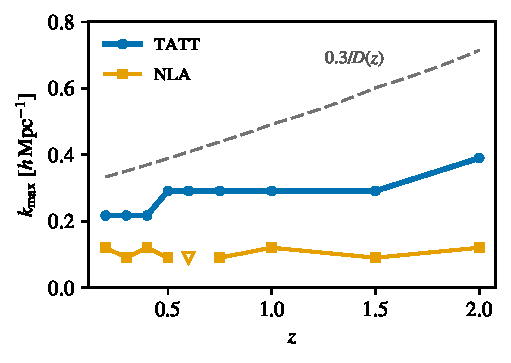
\includegraphics[width=3.5in]{plots/sim_cuts/sim_cuts.pdf}
  \caption{The goodness-of-fit scale cut of each model in FLAMINGO at
    the core snapshots. Color, line width and marker: the model; open
    triangle: a cut below the first grid node, $k = 0.09\hMpc$; gray
    dashed: the production mask $\kuv = 0.3/D(z)$.}
  \label{fig:simcuts}
\end{figure}

Two properties of the rule matter for how it is used. First, it is
noisy: when the truth is the model itself plus FLAMINGO noise, a
snapshot cuts anyway in \FalseNLA\% (NLA) and \FalseTATT\% (TATT) of
the realizations, so per-snapshot cuts are smoothed in $z$ rather than
read one by one. Second, and decisive, it is a significance, so it
depends on the box. With the residual fixed, a box of $f$ times the
volume has errors $\sigma/\sqrt f$ and an expected $\chi^2 \simeq \nu +
f\,\hat\lambda$, with $\hat\lambda = \chi^2_{\rm meas} - \nu$ the
measured excess. Figure~\ref{fig:volume} applies the same rule to
that expectation: a larger box rejects both models at smaller $k$,
without limit. The ratio of Roman's $\dchi$ to FLAMINGO's for the
actual residuals is 0.02 to 0.04, so Roman sees them as a box of
$f = 0.02$ to $0.04$ would; there the rule gives \VolNLAlo{} to
\VolNLAhi{} for NLA and \VolTATTlo{} to \VolTATThi{} for TATT. The
simulation cuts are the range of validity of each model in this box,
which an IA paper reports; they are evidence for the Roman cut, not
the cut.

\begin{figure}[tbp]
  \centering
  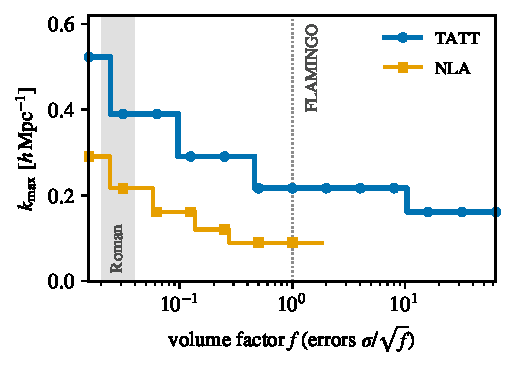
\includegraphics[width=3.5in]{plots/cut_volume/cut_volume.pdf}
  \caption{The goodness-of-fit cut, combined over the core snapshots,
    against the volume factor $f$ of the simulation. Color, line width
    and marker: the model; markers on every fourth value of $f$. Gray
    band: the $f$ at which FLAMINGO sees the residuals as Roman does;
    dotted: FLAMINGO itself. Where a curve ends, the cut lies below the
    first grid node.}
  \label{fig:volume}
\end{figure}

\section{The white II excess}
\label{sec:white}

FLAMINGO's II spectrum has a component that no single-tidal-field
model can produce. If GI and II both come from one tidal field, as in
NLA and at leading order in TATT, then $P_{EE}\PNL = \PdE^2$, so
\begin{equation}
  X(k) \equiv \left(P_{EE} - N_s\right) - \frac{\PdE^2}{\PNL}
\end{equation}
vanishes. In FLAMINGO it is flat in $k$ from 0.07 to $0.5\hMpc$ at
every snapshot and equals \WhiteLo{} to \WhiteHi{} times $N_s$
(Figure~\ref{fig:white}). The E-mode white power exceeds the B-mode
white power, so this is small-scale (one-halo-like) alignment, not
shape noise. Any one-halo alignment term tends to a constant as $k \to
0$, so a white spectrum is its leading form.

\begin{figure}[tbp]
  \centering
  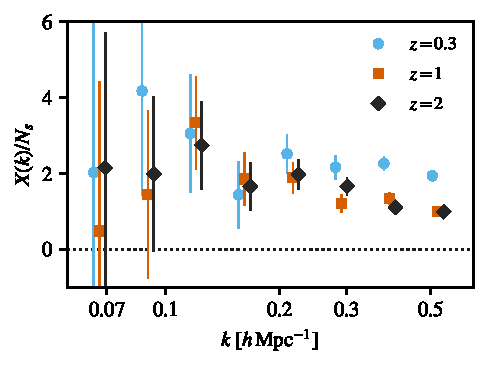
\includegraphics[width=3.5in]{plots/white_excess/white_excess.pdf}
  \caption{The white II excess $X(k)$ in units of the shape-noise level
    $N_s$ at three redshifts, with the FLAMINGO error bars; points are
    offset slightly in $k$. Dotted: $X = 0$, the value of any model in
    which GI and II come from one tidal field.}
  \label{fig:white}
\end{figure}

Its Roman signature follows in two lines. A white $P_{EE} = X$ gives,
through the Limber integral, a constant angular power $C = X\int
d\chi\, n_i n_j/\chi^2$, and the Hankel transforms of a constant are
\begin{equation}
  \xi_+(\theta) = \int\frac{\ell\,d\ell}{2\pi}\,J_0(\ell\theta)\,C = 0
  \quad(\theta > 0),\qquad
  \xi_-(\theta) = \int\frac{\ell\,d\ell}{2\pi}\,J_4(\ell\theta)\,C =
  \frac{2C}{\pi\theta^2}.
\end{equation}
The term lives in $\xi_-$ at every angle: in the lowest tomographic
bin it is $2\sigma$ at 63 arcmin and $1\sigma$ at 116 arcmin. A mask
built from $\kuv$ removes small angles, not the large-angle tail, and
this is why the next section finds a bias that cutting cannot remove.

\section{What Roman requires, and why cutting does not remove the bias}
\label{sec:floor}

Two calculations turn the simulation residuals into survey terms.
The first asks how accurate the IA spectra must be. A coherent
fractional error $\varepsilon$ in GI or II at every $k' \ge k$ is
propagated to $\xi_\pm$ with the cell Jacobian, and $\varepsilon$ is
raised until $\dchi_{\rm Roman} = 1$ on the $K_0 = 0.3$ mask. Roman
requires GI to \ReqGIa\% above $k = 0.12$, \ReqGIb\% above 0.29 and
\ReqGIc\% above $0.52\hMpc$, and II to \ReqIIa, \ReqIIb{} and
\ReqIIc\%. Figure~\ref{fig:required} compares this with the error of
each model fitted to FLAMINGO at $k \le 0.16$: on average GI is within
the requirement for both models, while NLA's II reaches it at $k \simeq
0.12$ and exceeds it from 0.29, because of the white term. The II spectrum, not
the shape of GI, is what matters for Roman.

\begin{figure}[tbp]
  \centering
  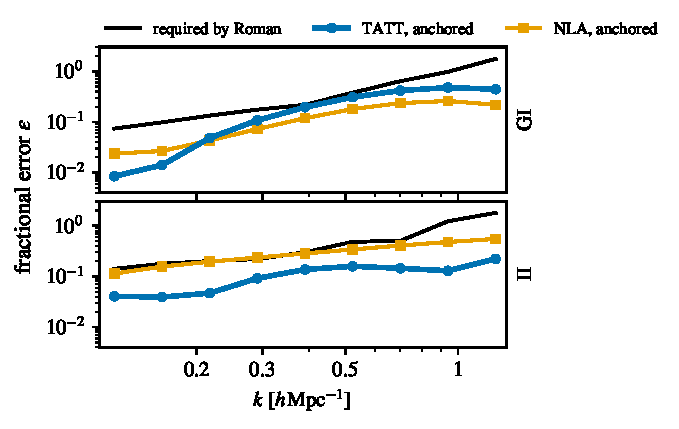
\includegraphics[width=3.5in]{plots/required_accuracy/required_accuracy.pdf}
  \caption{The fractional accuracy Roman requires of the IA spectra
    (black: a coherent error at every $k' \ge k$ worth $\dchi_{\rm
    Roman} = 1$ on the $K_0 = 0.3$ mask, Gaussian covariance) against
    the error of each model fitted to FLAMINGO at $k \le 0.16\hMpc$
    (mean over the core snapshots). Upper panel GI, lower panel II.
    The requirement relaxes by a factor of about 1.5 from $K_0 = 0.4$
    to 0.2.}
  \label{fig:required}
\end{figure}

The second follows the shift itself. Figure~\ref{fig:floor} places
every mask of the three families at its precision $\sigma(S_8)$ and its
figure of bias. The masks follow curves of constant absolute shift:
$|\delta S_8|$ stays between \FloorLo{} and $\FloorHi\times10^{-3}$
while $\sigma(S_8)$ changes by a factor of \SigmaRange. Cutting does not
reduce the shift; it enlarges the error bar until the shift is no
longer significant. A threshold on the figure of bias is therefore a
threshold on $\sigma(S_8)$: with the white term in the truth, a
stricter budget can only be met by discarding precision. At equal bias
the $1/D(z)$ family is the most precise, by 15 to 25\%, because it cuts
hardest at low redshift, where the white tail of the low-redshift bins
is largest.

\begin{figure}[tbp]
  \centering
  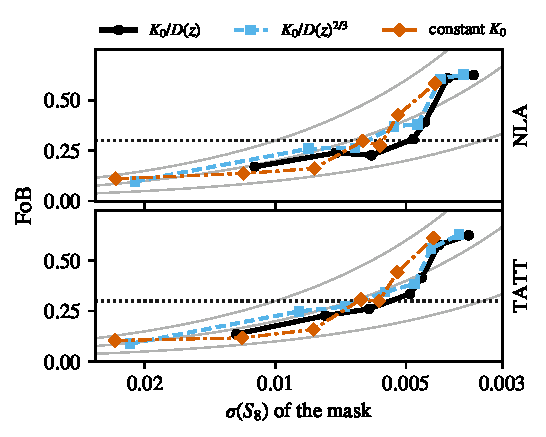
\includegraphics[width=3.5in]{plots/bias_floor/bias_floor.pdf}
  \caption{The figure of bias of every mask against its precision
    $\sigma(S_8)$ (Gaussian covariance, case A), precision increasing
    to the right; NLA above, TATT below. Color, line width, marker and
    line style: the redshift shape of the mask. Thin gray: constant
    $|\delta S_8| = 1$, 2 and $3\times10^{-3}$, bottom to top; dotted:
    $\FoB = 0.3$.}
  \label{fig:floor}
\end{figure}

\section{The cut with the production covariance}
\label{sec:cut}

Figure~\ref{fig:fob} is the result the paper uses. With the white term
left in the truth (solid), NLA and TATT behave alike in the $1/D(z)$
family: $\FoB = \ExNLAthreeFoB$ and \ExTATTthreeFoB{} at $K_0 = 0.3$,
\ExNLAfiveFoB{} and \ExTATTfiveFoB{} at 0.35, and both fail at 0.4.
TATT's better description of FLAMINGO does not reduce its bias,
because the bias comes from the white term that neither model has.
With one free white-II amplitude (dashed), the floor disappears and
the models separate: NLA reaches \ExNLAwFour{} at $K_0 = 0.4$ while
TATT stays below 0.25 to $K_0 = 0.5$. The amplitude costs at most 3\%
in $\sigma(S_8)$ with this covariance. A constant cut separates the
models by one step even without it: NLA passes to $\kuv = 0.35$ and
TATT to 0.4.

\begin{figure}[tbp]
  \centering
  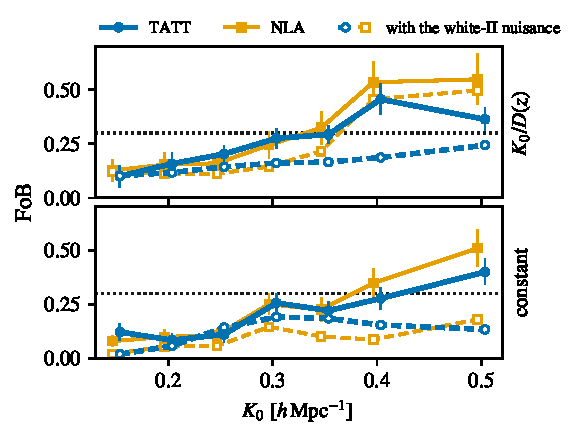
\includegraphics[width=3.5in]{plots/fob_k0/fob_k0.pdf}
  \caption{The Roman figure of bias against the cut, production
    covariance, FLAMINGO IA injected. Upper panel: $\kuv = K_0/D(z)$;
    lower: a constant $\kuv = K_0$. Color, line width and marker: the
    model; solid, filled, with the FLAMINGO-noise error bars: case A;
    dashed, open: case A with one free white-II amplitude; dotted:
    $\FoB = 0.3$. Case B agrees with case A to within the error bars.
    NLA and TATT are offset slightly in $K_0$. \kuvclause}
  \label{fig:fob}
\end{figure}

The production covariance is larger than the Gaussian one, so at the
same absolute shift every crossing moves outward, as the bias floor
predicts: with the Gaussian covariance both models cross 0.3 at $K_0
\simeq \GaussKzero$.
Table~\ref{tab:rec} collects the configurations that pass.

\begin{table}[tbp]
  \centering
  \small
  \caption{Cut configurations that keep $\FoB < 0.3$ with the
    production covariance (case A, case B in brackets; $\sigma(S_8)$ of
    case A). Separate $\xi_\pm$: the $\xi_+$ rows cut at $K_0^+$, the
    $\xi_-$ rows at $K_0^-$, both $1/D(z)$.}
  \label{tab:rec}
  \begin{tabular}{llccc}
    \toprule
    configuration & model & cosmic-shear cut & points & FoB \\
    \midrule
    with the white-II amplitude & NLA & $K_0 = 0.35$, $1/D$ & 317 & 0.22 \\
     & TATT & $K_0 = 0.5$, $1/D$ & 385 & 0.24 \\
    constant cut & NLA & $\kuv = 0.35$ & 266 & 0.22 (0.19) \\
     & TATT & $\kuv = 0.4$ & 292 & 0.28 (0.28) \\
    separate $\xi_\pm$ & NLA & $K_0^+ = 0.35$, $K_0^- = 0.3$ & 306 & 0.28 (0.27) \\
     & TATT & $K_0^+ = 0.4$, $K_0^- = 0.3$ & 315 & 0.27 (0.25) \\
    common $1/D$ & both & $K_0 = 0.3$ & 281 & 0.24 / 0.28 \\
    \bottomrule
  \end{tabular}
\end{table}

\section{A halo model with central alignment}
\label{sec:hmc}

NLA, TATT and the satellite model of Fortuna et al.\ (2021) all place
the GI of central galaxies on $\PNL$, which assumes every central is
perfectly aligned with the matter of its own halo. FLAMINGO's $P_{hE}$
lies 20 to 40\% below that prediction at $k = 0.5$ to $1.3\hMpc$. The
halo model HMc splits the term into a two-halo piece (centrals aligned
with the tidal field of other halos, on $I_1(k)P_{\rm lin}$) and a
central one-halo piece, in which each central follows the quadrupole of
its own elliptical NFW host with literature halo shapes and one free
alignment strength $a_c$; satellites follow Fortuna et al.\ (2021). With a
free white term $W$ in both models, the summed $\chi^2/\nu$ at $\kmax =
0.52\hMpc$ over the core is \HMcChi{} for HMc against \HMcTATTChi{}
for TATT, and the goodness-of-fit cuts move to \HMcCutLo{} to
\HMcCutHi$\hMpc$ at every snapshot.

In Roman (Figure~\ref{fig:hmc}, case B), HMc keeps the figure of bias
at or below \HMcMaxFoB{} to $K_0 = 0.5$ in both families, while TATT
crosses 0.3 at $K_0/D(z) = \HMcTATTcrossD$ and at a constant
$\HMcTATTcrossC$. On Roman's masks $a_c$ is unconstrained (often at
zero), so the gain there comes mostly from moving the two-halo terms
from $\PNL$ to $I_1 P_{\rm lin}$ and $P_{\rm lin}$. The HMc templates
are evaluated at the fiducial cosmology.

\begin{figure}[tbp]
  \centering
  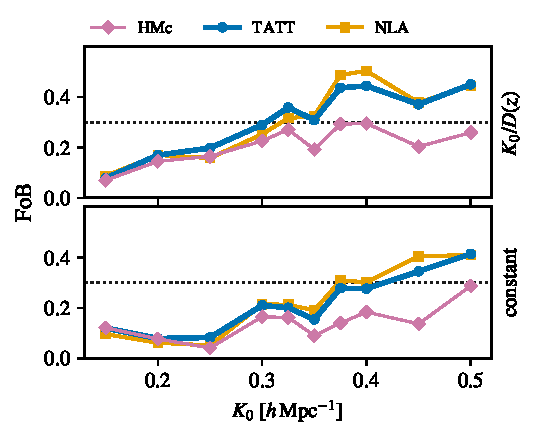
\includegraphics[width=3.5in]{plots/hmc_fob/hmc_fob.pdf}
  \caption{The Roman figure of bias of NLA, TATT and the halo model with
    central alignment (HMc), production covariance, case B, no white-II
    amplitude. Upper panel: $\kuv = K_0/D(z)$; lower: constant. Color,
    line width and marker: the model; dotted: $\FoB = 0.3$. FLAMINGO-noise
    uncertainties are 0.03 to 0.08. \kuvclause}
  \label{fig:hmc}
\end{figure}

\section{Recommendation and wording for the paper}
\label{sec:rec}

The defining criterion is the Roman one of Section~\ref{sec:setup},
applied to each model separately, with the $1/D(z)$ masks; the
simulation cuts, the volume argument and the required accuracy are
the supporting evidence. Nothing requires the two models to share a
cut, and the difference between them appears once the white term is
modelled. The recommended set is the first row pair of
Table~\ref{tab:rec}. For the lens probes, keep sources behind lenses
and $K_0^{\rm ggl} = K_0^{\rm gc} = 0.2$; the 3x2pt bias is then set
by the cosmic-shear cut (appendix ``\nameref{app:lens}''). A paragraph for the
methods section:

\begin{quote}
  \small
  We define the cosmic-shear scale cuts with the IR/UV decomposition
  of arXiv:2603.13031: an angular bin of $\xi_\pm^{ij}$ is kept if the
  fraction of its signal from wavenumbers $k > \kuv(z) = K_0/D(z)$ is
  below $\alpha = 0.05$. We fix $K_0$ separately for each IA model with
  an injection test: the Roman data vector is computed with the GI and
  II spectra measured in FLAMINGO, the analysis model is fitted with
  all cosmological and nuisance parameters free, and $K_0$ is the
  largest value for which the shift of the maximum-posterior $(\Omega_m,
  S_8)$ stays below $0.3\sigma_{\rm 2D}$, after verifying that the same
  test on a data vector generated with the analysis model returns zero.
  The FLAMINGO spectra contain a white (one-halo) E-mode alignment term
  that neither model includes and that contributes to $\xi_-$ on all
  angular scales; we model it with one free amplitude in both analyses.
  NLA then requires $K_0 = 0.35\hMpc$, while TATT remains unbiased to
  $K_0 = 0.5\hMpc$, which keeps \ExGainPts\% more data points and
  reduces $\sigma(S_8)$ by \ExGainSig\%.
\end{quote}

\appendix

\section{Method details}
\label{app:method}

\paragraph{Why the MAP shift.}
At $K_0 = 0.3$ an MCMC reproduces the linearized MAP shifts, and the
matched TATT control, which has zero MAP shift, has a posterior-mean
shift of \Projection$\sigma$: the prior volume of the weakly
constrained $\eta_2$ and $b_{\rm TA}$. The criterion is therefore stated
for the MAP, or for the posterior mean minus the matched control;
otherwise TATT is charged with a projection effect that is not model
failure.

\paragraph{The threshold.}
A shift of $b\sigma$ in one parameter lowers the coverage of the 68\%
interval to $\Phi(1-b) - \Phi(-1-b)$: 0.683, 0.661 and 0.625 for $b =
0$, 0.3 and 0.5. The 0.3 of DES Y3 was a budget for all modelling
systematics together; an equal share in quadrature among IA, baryons
and nonlinear bias would give IA $0.3/\sqrt3 = 0.17$, which no useful
mask meets while the white term is in the truth
(Section~\ref{sec:floor}).

\paragraph{Separate cuts for $\xi_+$ and $\xi_-$.}
The bias lives in $\xi_-$ (the white term is invisible in $\xi_+$),
and $\xi_+$ separates the models: with $\xi_-$ restricted, NLA fails
between $K_0^+ = 0.35$ and 0.4, where the GI dip of $\PdE/\PNL$ at
$k \simeq 0.3$ to 1 enters, which TATT follows. At equal bias separate
cuts are 13 to 20\% more precise than a common cut, at the price of a
second free number per probe.

\paragraph{Theory-error covariance.}
Adding the measured model error to the covariance, $C \to C +
\mathsf{J}\Sigma_{\rm th}\mathsf{J}\T$, lowers the figure of bias by 15
to 40\% but leaves the shift in units of the statistical error
unchanged, because the bias comes from low $k$, where the measured
envelope is a few percent. With an envelope from one simulation it
behaves like a softer cut.

\section{Lens probes}
\label{app:lens}

With sources behind lenses (28 lens-source pairs), the GI term in
$\gamma_t$ is small: galaxy-galaxy lensing plus clustering alone stays
at or below $0.2\sigma$ for both models to $K_0^{\rm ggl} = 0.2$, and in
3x2pt the bias is set by the cosmic-shear cut. With all pairs, the
same-bin $\gamma_t^{ii}$ measures $\PdE$ directly; NLA then stays
below $0.3\sigma$ only for $K_0^{\rm ggl} \lesssim 0.15$, and TATT stays below $0.2\sigma$ only
through a solution at the $\eta_2$ prior bound driven by the $z \ge
1.5$ snapshots. Clustering carries no IA; $K_0^{\rm gc} = 0.2$ is set
by the galaxy-bias modelling.

\section{Numerical checks}
\label{app:checks}

\begin{itemize}\sloppy
  \item cosmolike: cocoa-cosmolike-core with \texttt{core-sim-IA.patch}
    and cocoa\_roman\_real with \texttt{roman\_real-sim-IA.patch}, both
    in \texttt{cosmolike\_patches/}, compiled with
    \texttt{-DSIM\_KMIN\_HMPC=1e-6 -DSIM\_KMAX\_HMPC=0} (the default
    build trims the tables to 0.5 to $7\hMpc$, which costs $\dchi \sim
    1000$).
  \item \texttt{example1.modelvector} is reproduced to $3\times10^{-5}$
    (median), reading the $n(z)$ with cocoa's left-edge convention.
  \item The conversion inside \texttt{sim\_IA.c} gives the same
    $\xi_{\rm IA}$ as the Python conversion to $2.5\times10^{-9}$; an
    NLA power law injected as tables matches native NLA to $\dchi =
    0.001$.
  \item Native TATT with $A_2 = b_{\rm TA} = 0$ equals native NLA
    exactly; linearized and fully nonlinear fits agree to every quoted
    digit.
  \item The FLAMINGO inputs in \texttt{flamingo/data/PS} reproduce the
    data arrays of \texttt{analysis/roman\_dchi2/v2/fits.npz} to
    $10^{-16}$ (checked 13 November 2026). Refitting with CAMB 1.6.7
    instead of the tested 2.0.5 changes $\PNL$ by 0.07\% (median), the
    fit $\chi^2$ by 0.4\% (median) and the degenerate TATT directions by
    more; the shipped \texttt{fits.npz} is the reference.
\end{itemize}

\section{Where the code and results are}
\label{app:code}

Paths relative to the repository root (\texttt{JerreYjz/ia-mismodeling}).

\begin{center}
  \small
  \begin{tabular}{ll}
    \toprule
    result & script $\rightarrow$ output \\
    \midrule
    FLAMINGO spectra & \texttt{flamingo/extraction/} $\rightarrow$ \texttt{flamingo/data/PS} \\
    conversion and fits & \texttt{analysis/roman\_dchi2/v2/fit\_models.py} $\rightarrow$ \texttt{v2/fits.npz} \\
    simulation cuts & \texttt{v3/v3\_flamingo.py} $\rightarrow$ \texttt{v3/cuts.csv} \\
    volume, calibration & \texttt{v4/sim\_strategies.py} $\rightarrow$ \texttt{v4/sim\_strategies.json} \\
    required accuracy, trade-off & \texttt{v4/roman\_strategies.py}, \texttt{plot\_strategies.py} \\
    Roman scans & \texttt{v3/mask\_scan.py} $\rightarrow$ \texttt{v3/mask\_scan\_ex1\_*.json} \\
    halo model & \texttt{v6/halo\_central\_fit.py}, \texttt{v6/hmc\_scan.py} \\
    this note's figure data & \texttt{notes/scale\_cuts\_summary/plots/make\_figure\_data.py} \\
    \bottomrule
  \end{tabular}
\end{center}

The work logs this note was rebuilt from stay in
\texttt{analysis/roman\_dchi2/report/}: \texttt{summary.pdf} (the
simulation fits, the Roman test, the mask families, GGL and 3x2pt with
the Gaussian covariance), \texttt{strategies.pdf} (every cut strategy,
with the production covariance), \texttt{hmc\_review.pdf} (the halo
model), \texttt{fob\_note.pdf} (how the figure of bias is computed) and
\texttt{stitched.pdf} (the stitched-truth control).

\section{Open issues}
\label{app:open}

\begin{itemize}
  \item The white term is either part of the truth or a nuisance of the
    model; together with whether separate $\xi_\pm$ cuts are acceptable,
    this choice selects the row of Table~\ref{tab:rec}.
  \item The cut rests on one simulation and one galaxy selection, so
    robustness to the IA truth is untested beyond the stitched-truth
    control, which is the optimistic bound.
  \item The chains at the chosen mask (MAP and control-subtracted
    posterior mean) have not been run with the cocoa likelihood.
  \item The survey settings behind \texttt{example1\_cov} are not
    documented in \texttt{cocoa\_roman\_real}.
  \item Several TATT fits sit at a prior bound ($b_{\rm TA} = 0$ with the
    white amplitude; $\eta_2$ in some case-A fits), and the $z = 2$
    snapshot flips to $A_2 > 0$.
  \item $\alpha = 0.05$ throughout; the second knob of the mask was not
    varied.
\end{itemize}

\end{document}
